% !TeX spellcheck = en_US
% !TeX encoding = UTF-8
% =============================

% ========== Classe do documento, geometria, codificação e versão
\documentclass[12pt]{article}
\usepackage[a4paper,top=2cm,bottom=2cm,left=2cm,right=2cm]{geometry} % marginparwidth=1.75cm
% ----------
\usepackage[utf8]{inputenc}
\usepackage[T1]{fontenc}
% ==========

% ========== Pacotes
\usepackage{FHZ-packages-minimum}
\usepackage{FHZ-packages-TikZ-mydef}
% ==========
\usepackage{enumitem}
\usepackage{paracol}
\usepackage{multicol}
\usepackage[]{animate} %draft
% ==========
\usepackage{abstract}
\renewcommand{\abstractnamefont}{\normalfont\Large\bfseries}
%\renewcommand{\abstracttextfont}{\normalfont\Huge}
% ==========

% ==========
\usepackage{FHZ-textos}
% ==========

% =================== Formatações e marca d'água em arquivos de estilos .sty
% ---------- Formatacao -- hf
\usepackage{FHZ-formatacao-hf-headings_h_R_thepage}
% ---------- Formatacao -- hyperref
\usepackage[07]{FHZ-formatacao-hyperref-opt}
% ===================

% ========== Novos comandos para inserir figuras e TikZ de forma padronizada
\usepackage{FHZ-figures-TikZ-IEEE}
% ==========

% ========== Capa
\usepackage{FHZ-capa-article}
% ==========

\usepackage{tikz-among-us}
\usepackage{tikz-among-us-fancyhdr}
\usepackage[cor=violet!70!white,BG,type=1]{tikz-among-us-watermark-eso-pic}

%\usepackage{FHZ-tcolorbox-01}

\usepackage{FHZ-listings-showexpl-style}
\lstset{style=estiloBaseGeral,
  frame=none,
  keywordstyle=\color{blue}
}

\usepackage[skins,listings,breakable,raster]{tcolorbox}
\tcbuselibrary{listings}

\newtcblisting{FHZtcbAmongUs}[1][]{ %
  enhanced,
  colback=cyan!5!white, colframe=violet!75!black, fonttitle=\large\bfseries,
  colbacktitle=violet!85!black,
  listing and text, breakable,
  after={\par\vspace{0.5\baselineskip}\noindent},
  listing options={style=estiloTcbAzul},
  #1
}

\newtcolorbox{FHZboxEnumerateStyle}{
  enhanced, breakable,
  colback=orange!15!white,
  colframe=orange!50!black,
  watermark tikz={\tikz
    \node[opacity=0.4, rotate around={-45:(1.75,2.3)}]{\amongUsOriginal{blue}{white}};
    \node[opacity=0.4, rotate around={45:(1.75,2.3)}] at (5,0) {\amongUsOriginal{pink}{white}};
    \node[opacity=0.4, rotate around={-135:(1.75,2.3)}] at (10,0) {\amongUsOriginal{green}{white}};
    \node[opacity=0.4, rotate around={135:(1.75,2.3)}] at (15,0) {\amongUsOriginal{olive}{white}{black}{white}};
  }
}
\newenvironment{FHZtcbEnumerate}{%
  \begin{FHZboxEnumerateStyle}\begin{enumerate}}
    {\end{enumerate}\end{FHZboxEnumerateStyle}
}

% ========== Dados capa folha rosto ========== Sempre crie uma cópia local
\newcommand{\edicao}{1}
\newcommand{\versao}{1.2.0}
% ======================
\newcommand{\textoEdicao}{Edition}
\newcommand{\textoVersao}{Version}
\newcommand{\textoCopyright}{}
% ======================
\newcommand{\Universidade}{}
\newcommand{\Curso}{} %{Curso --}
\newcommand{\Departamento}{}
% ---
\newcommand{\AutorA}{\textbf{FHZ}}
\newcommand{\AutorB}{}
\newcommand{\AutorC}{}
\newcommand{\AutorD}{}
% ---
\newcommand{\Titulo}{\textbf{There is a {\TikZ}-Impostor Among us}}
% ---
\newcommand{\Cidade}{\textbf{tikz-among-us package}\\} %{Cidade --}
\newcommand{\Estado}{\url{https://www.ctan.org/pkg/tikz-among-us}\\} %{Estado --}
\newcommand{\Pais}{\textbf{Brasil} -- \textbf{{\today} -- \textoVersao: \versao}}
\newcommand{\Mes}{}
\newcommand{\Ano}{}
% ---
\newcommand{\de}{}
% ---
\newcommand{\textoFolhaRosto}{%
}
% ---
\newcommand{\OrientadorA}{}
\newcommand{\OrientadorB}{}
\newcommand{\textoOrientador}{}
\newcommand{\textoCoOrientador}{}
% ====================== Input_Folha_Rosto_Livro_Versao

% ========== Hypersetup local
\hypersetup{pdfinfo={
		Title={\Titulo},
		Author={\AutorA} %,\AutorB
}}
% ==========

\begin{document}
% ========== Capas
{\FHZCapaArticleCabecalho}
% ==========

\begin{abstract}
  \begin{FHZboxEnumerateStyle}
    This is the \texttt{tikz-among-us} package documentation. This package recreates some AmongUs characters in {\TikZ} environment. Some interesting uses alongside other packages are also presented.
  \end{FHZboxEnumerateStyle}
\end{abstract}

\begin{FHZboxEnumerateStyle}
  \begin{multicols}{2}
    {\small \tableofcontents}
  \end{multicols}
\end{FHZboxEnumerateStyle}
\section{Introduction}

The following packages are used in the examples and applications.
\begin{FHZtcbEnumerate}
  \item \href{https://www.ctan.org/pkg/tikz}{{\CTAN} -- tikz}

  Whose following packages are always used as reference of quality and capabilities:
  \begin{enumerate}
    \begin{multicols}{2}
      \item \href{https://www.ctan.org/pkg/tikzducks}{{\CTAN} -- tikzducks}
      \item \href{https://www.ctan.org/pkg/tikzmarmots}{{\CTAN} -- tikzmarmots}
    \end{multicols}
  \end{enumerate}
  \begin{multicols}{2}
%    \item \href{https://www.ctan.org/pkg/adjustbox}{{\CTAN} -- adjustbox}
    \item \href{https://www.ctan.org/pkg/tcolorbox}{{\CTAN} -- tcolorbox}
    \item \href{https://www.ctan.org/pkg/fancyhdr}{{\CTAN} -- fancyhdr}
    \item \href{https://www.ctan.org/pkg/eso-pic}{{\CTAN} -- eso-pic}
    \item \href{https://www.ctan.org/pkg/animate}{{\CTAN} -- animate}
  \end{multicols}
\end{FHZtcbEnumerate}

The basic concept started as a question at {\TeXStackExchange} and after some research some new ideas have been found to improve the initial sketch.
\begin{FHZtcbEnumerate}
  \item \href{https://tex.stackexchange.com/questions/567009/there-is-a-tikz-impostor-among-us/567010#567010}{{\TeXStackExchange} -- There is a TikZ-impostor Among us}: is the original post which started with a very simple design and then received an update with the shade-command style derived from:
  \begin{enumerate}
    \item \href{https://tex.stackexchange.com/questions/424113/how-to-use-tikz-shade-command-in-order-to-achieve-3d-like-results}{{\TeXStackExchange} -- How to use Tikz {\textbackslash}shade command in order to achieve 3D like results}: is the inspiration to create commands with parts of a drawing to build a greater design in {\TikZ} and the command shade.
    \item \href{https://youtu.be/1zZZBB9-Nm8}{{\YouTube} -- MatPat's Game Theory}: is the inspiration to the design of the shadow. Many artists have replicated the original design of the game.
    \item \href{https://youtu.be/yZrhRKyFP-U}{{\YouTube} -- Game Toons -- Among Us Logic Movie | Cartoon Animation}: is a animation featuring Among Us characters and source to many emotional expressions and hand positions since many of them are used to make characters much more expressive.
  \end{enumerate}
\end{FHZtcbEnumerate}

The original game is available in different online stores. I don't own the game, or have any relationship with authors nor any enterprise. I'm just a guy who liked the game and used it as a motivation to create a package for {\TikZ} users.
\begin{FHZtcbEnumerate}
  \item \href{https://play.google.com/store/apps/details?id=com.innersloth.spacemafia&hl=pt_BR&gl=US}{AmongUs original game to smartphones}
\end{FHZtcbEnumerate}

\section{Using the package}

There are three base style files.
\begin{FHZtcbAmongUs}[listing only]
\usepackage{tikz-among-us}
\usepackage{tikz-among-us-fancyhdr}
\usepackage{tikz-among-us-watermark-eso-pic}
\end{FHZtcbAmongUs}

A brief description follows:
\begin{FHZtcbEnumerate}
  \item \verb|\usepackage{tikz-among-us}|: Main \texttt{.sty} file with the definitions in {\TikZ} of each body part, style of shading and complete design. Although this style is far from the utmost best standards for a {\TikZ} package, it has been a very useful project to motivates me to learn more and improve my own usage of {\TikZ} beyond standalone applications or drawings and also my very first {\CTAN} publication.

  \item \verb|\usepackage{tikz-among-us-fancyhdr}|: A basic implementation to add the Among Us characters in headers or footers due the \texttt{fancyhdr} package. This is not a final super fancy implementation, but it splits the configurations to a separated \texttt{.sty} file, which can be edited aownernd reused.

  \item \verb|\usepackage{tikz-among-us-watermark-eso-pic}|: A preset implementation of watermarks using the \texttt{eso-pic} package. This implementation takes advantage of the \texttt{kvoptions} packages in order to add some degrees of flexibility to the watermarks. Of course anyone could just replace the basic command from \texttt{eso-pic} in each file they want. The preset configurations aim to be a synthesis and make its usage a little bit more flexible than just copying and pasting content in each file.
\end{FHZtcbEnumerate}

\section{Examples -- tikz-among-us}

While creating the drawing, I did a first attempt, now called \texttt{Original}, which is a command with a \texttt{tikzpicture} inside it. This command was not made with the best method to be flexible, but it is indeed very simple and direct. I chose to keep it as an alternative to the new commands and because it has a different style.
The are two main styles, \texttt{Style I} and \texttt{Style II}. \texttt{Style I} has the shadow create by ``hand'', it means, the shadow is a fixed perspective which boundaries were directly programmed in {\TikZ}. \texttt{Style II} uses the library \texttt{shade} to create shadows, but I couldn't reproduced the same result as I did in \texttt{Style I}.
In this sense, I chose to keep both styles and using the roman number as a suffix of each command.

\subsection{Styles I e II}

The basic syntax to insert each character is:
\begin{FHZtcbAmongUs}[listing only]
\amongUsI[<options>]{<BodyColor>}{<EyeColor>}
\end{FHZtcbAmongUs}
\noindent
and for each body part, the commands are:
\begin{FHZtcbAmongUs}[listing only]
\amongUsBackpackI[<options>]{<BodyColor>}
\amongUsBodyI[<options>]{<BodyColor>}
\amongUsEyesI[<options>]{<EyeColor>}
\end{FHZtcbAmongUs}
\noindent
where \texttt{<options>} is any suitable option of the environment \texttt{scope} of {\TikZ}; and \texttt{<BodyColor>} and \texttt{<EyeColor>} are any color provided such as {\TikZ} recognizes them.
For each basic command with suffix \texttt{I} there is another command with suffix \texttt{II}, that represents the alternative method to create shades. There are no \texttt{Style II} for every design.

This is the basic use of the package.

\begin{paracol}{2}
\begin{FHZtcbAmongUs}[title=Basic Use -- Style I]

\begin{tikzpicture}
  \amongUsI{yellow}{cyan}
\end{tikzpicture}
\end{FHZtcbAmongUs}
\switchcolumn
\begin{FHZtcbAmongUs}[title=Basic Use -- Style II]
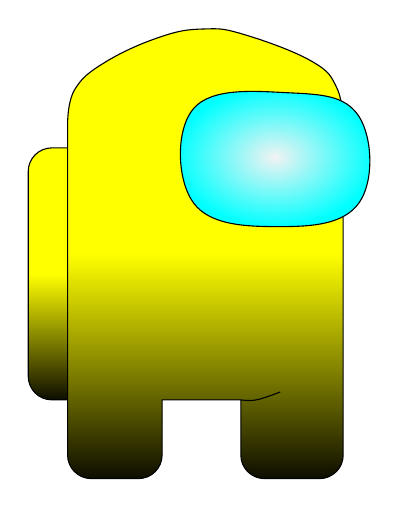
\begin{tikzpicture}
  \amongUsII{yellow}{cyan}
\end{tikzpicture}
\end{FHZtcbAmongUs}
\end{paracol}

Each body part was created to have its coordinate origin such as it is corrected placed on the main body without the need of any shift.
On the other hand, the \texttt{shift=\{(x,y)\}} command of the environment \texttt{scope} is a well suitable method to move each part.

\begin{paracol}{2}
\begin{FHZtcbAmongUs}[title=Each body part -- Style I]
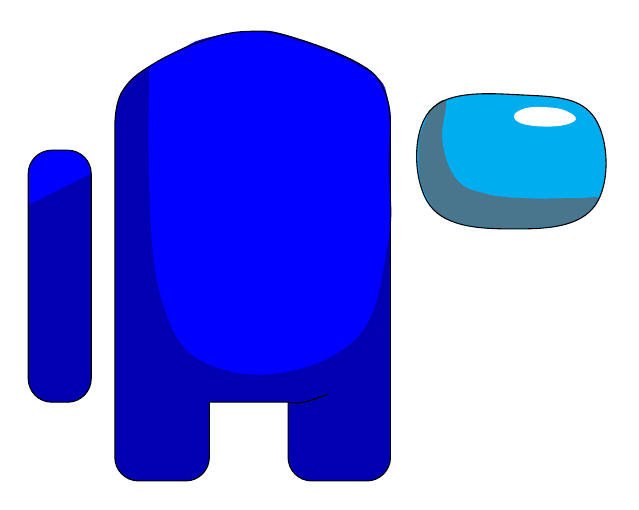
\begin{tikzpicture}
  \amongUsBackpackI
    [shift={(0,0)}]{blue}
  \amongUsBodyI
    [shift={(0.6,0)}]{blue}
  \amongUsEyesI
    [shift={(3,0)}]{cyan}
\end{tikzpicture}
\end{FHZtcbAmongUs}
\switchcolumn
\begin{FHZtcbAmongUs}[title=Each body part -- Style II]

\begin{tikzpicture}
  \amongUsBackpackII
    [shift={(0,0)}]{green}
  \amongUsBodyII
    [shift={(0.6,0)}]{green}
  \amongUsEyesII
    [shift={(3,0)}]{red}
\end{tikzpicture}
\end{FHZtcbAmongUs}
\end{paracol}

%Unfortunately, I'm (still) not the most proficient {\TikZ} user, so I didn't create the most optimized style to properly use the command \texttt{scale}, therefore, it is suggested to use the command \texttt{{\textbackslash}adjustbox} from the package \texttt{adjustbox} to scale the drawing without incurring in some errors with the \texttt{rounded corners} used in the design.

After learning the issues between \texttt{scale} and \texttt{rounded corners}, I update the drawing since version \texttt{1.1.0} to work with the \texttt{scale} options. Despite the update, the alternative method using the command \texttt{{\textbackslash}adjustbox} from the package \texttt{adjustbox} is still a valid option.
To rotate the draw around its center the command \texttt{rotate around=\{angle:(x0,y0)\}} should be used. The center of mass is close to the coordinates $x_0 = 1.75$ and $y_0 = 2.3$.

\begin{FHZtcbAmongUs}[title=Scaling with scale, sidebyside, righthand ratio=0.40]
  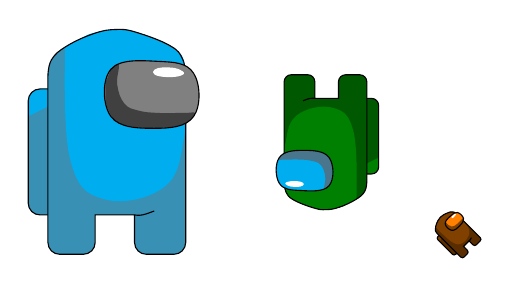
\begin{tikzpicture}
    \amongUsI[scale=0.5]{cyan}{gray}
    \amongUsI[scale=0.3, shift={(10,3)},
      rotate around={180:(1.75,2.3)}]
        {green!50!black}{cyan}
    \amongUsI[scale=0.1, shift={(50.5,0)},
      rotate around={45:(1.75,2.3)}]
        {orange!50!black}{orange}
  \end{tikzpicture}
\end{FHZtcbAmongUs}

\subsection{Style -- Original}

The original design is much more simplistic.

\begin{FHZtcbAmongUs}[title=Original Design -- Inside \textit{tikzpicture}]
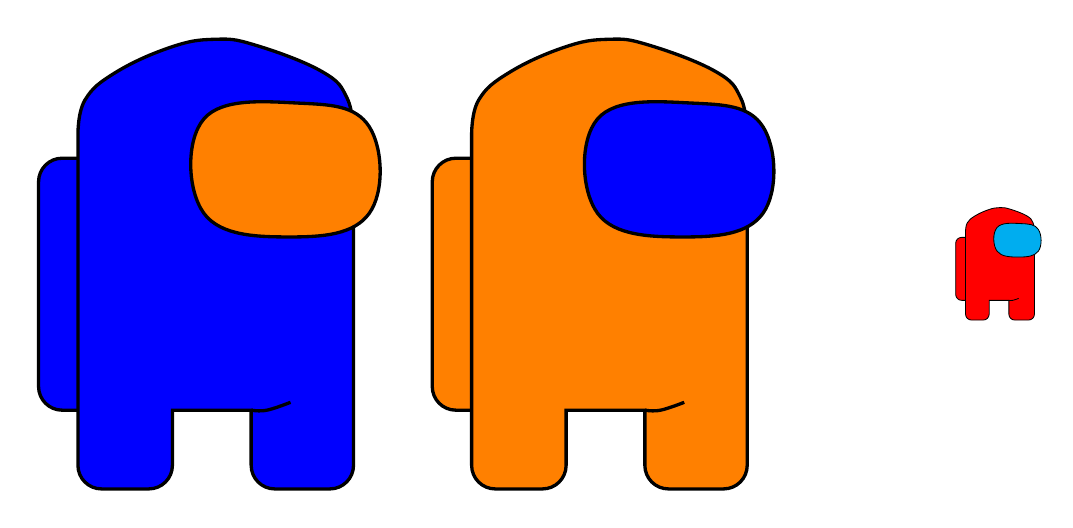
\begin{tikzpicture}
  \node at (0,0) {\amongUsOriginal{blue}{orange}};
  \node at (5,0) {\amongUsOriginal{orange}{blue}};
  \node[scale=0.25] at (10,0) {\amongUsOriginal{red}{cyan}};
\end{tikzpicture}
\end{FHZtcbAmongUs}

Although it is simplistic, it was a good start point to insert emotions as options to the style. The emotions shall be added to \texttt{Styles I} and \texttt{II} in the future. The \texttt{Original} style can be use outside a \texttt{tikzpicture} environment.

\begin{FHZtcbAmongUs}[title=Original Design -- Outside \textit{tikzpicture}]
\amongUsOriginal{black}{cyan}
\amongUsOriginal[angry]{gray}{cyan}
\amongUsOriginal[very angry]{white}{cyan}
\end{FHZtcbAmongUs}

Inside the \texttt{tikzpicture} environment is possible to use some options of the command \texttt{node} to produce some more combinations. Indeed, that's the best method to achieve a black body suit with visible lines.

\begin{FHZtcbAmongUs}[title=Original Design -- Inside \textit{tikzpicture} with \textit{node} options]
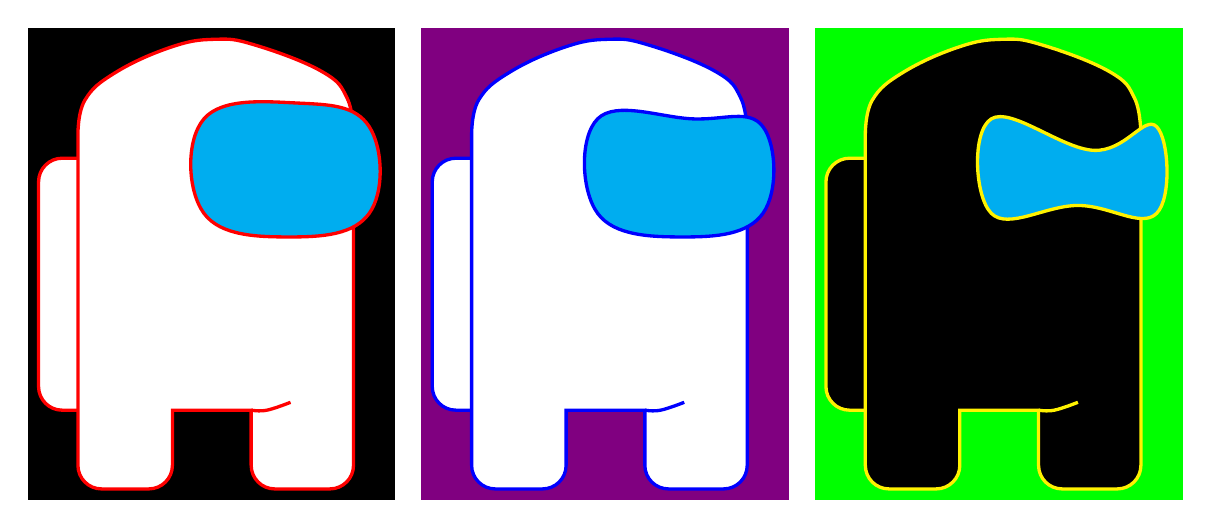
\begin{tikzpicture}[every path/.style={very thick}]
  \node[red, fill=black] at (0,0) {\amongUsOriginal{white}{cyan}};
  \node[blue, fill=violet] at (5,0) {\amongUsOriginal[angry]{white}{cyan}};
  \node[yellow, fill=green] at (10,0)
    {\amongUsOriginal[very angry]{black}{cyan}};
\end{tikzpicture}
\end{FHZtcbAmongUs}

\subsection{Show me your Hands}

The following command is used to present some hands
\begin{FHZtcbAmongUs}[listing only]
\amongUsHands<X>[<options>]{HandColor}
\end{FHZtcbAmongUs}
\noindent
where <X> is a letter from $A$ to $G$.

\begin{FHZtcbAmongUs}[title=Hands]

\begin{tikzpicture}[every path/.style={very thick}]
  \amongUsHandsA[shift={(0,0)}]{yellow}
  \amongUsHandsB[shift={(2,0)}]{red}
  \amongUsHandsC[shift={(4,0)}]{blue}
  \amongUsHandsD[shift={(6,0)}]{green!50!black}
  \amongUsHandsE[shift={(8,0)}]{orange}
  \amongUsHandsF[shift={(10,0)}]{violet}
  \amongUsHandsG[shift={(12,0)}]{gray}
\end{tikzpicture}
\end{FHZtcbAmongUs}

\subsection{Smile as an Impostor}

The following commands are used to create the impostor design
\begin{FHZtcbAmongUs}[listing only]
\impostorSmile[<options>]{SmileColor}
\impostorTeethUp[<options>]{SmileColor}
\impostorTeethLw[<options>]{TeethColor}
\impostorTeeth[<options>]{TeethColor}
\impostorI[<options>]{BodyColor}{EyeColor}{SmileColor}{TeethColor}
\impostorII[<options>]{BodyColor}{EyeColor}{SmileColor}{TeethColor}
\end{FHZtcbAmongUs}

There are two separated commands to draw the teeth in order to give some flexibility to new designs. The command \verb|\impostorTeeth| just call both commands and is used by the command \verb|\impostorI|.

\begin{FHZtcbAmongUs}[title=Why so serious? Smile!]
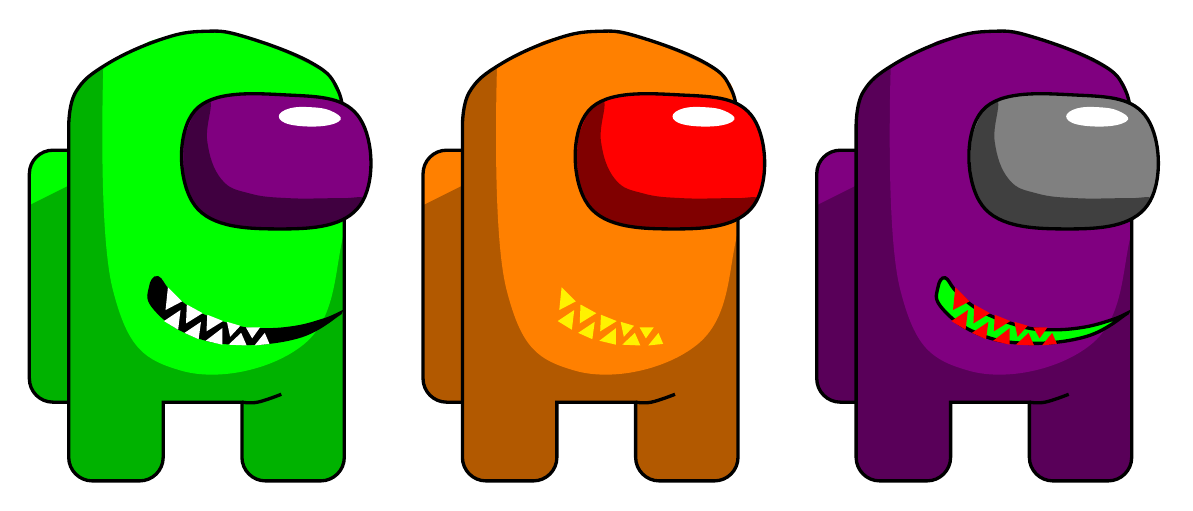
\begin{tikzpicture}[every path/.style={very thick}]
\amongUsI[shift={(5,0)}]{green}{violet}
\impostorSmile[shift={(5,0)}]{black}
\impostorTeethUp[shift={(5,0)}]{white}
\impostorTeethLw[shift={(5,0)}]{white}

\amongUsI[shift={(10,0)}]{orange}{red}
\impostorTeeth[shift={(10,0)}]{yellow}

\impostorI[shift={(15,0)}]{violet}{gray}{green}{red}
\end{tikzpicture}
\end{FHZtcbAmongUs}

\subsection{There are emotions on your Eyes}

The options to draw emotional eyes are:
\begin{FHZtcbAmongUs}[listing only]
\amongUsEyesAngryI[<options>]{EyeColor}
\amongUsEyesVeryangryI[<options>]{EyeColor}
\amongUsEyesHappyI[<options>]{EyeColor}
\amongUsEyesScaredI[<options>]{EyeColor}
\end{FHZtcbAmongUs}
\noindent
and respective \texttt{Style II} version.

\begin{FHZtcbAmongUs}[title=Are you angry?]

\begin{tikzpicture}[every path/.style={very thick}]
  \amongUsBackpackI{yellow}
  \amongUsBodyI{yellow}
  \amongUsEyesAngryI{cyan}

  \begin{scope}[shift={(5,0)}]
    \amongUsBackpackI{red}
    \amongUsBodyI{red}
    \amongUsEyesVeryangryI{blue}
  \end{scope}

  \begin{scope}[shift={(10,0)}]
    \amongUsBackpackI{blue}
    \amongUsBodyI{blue}
    \amongUsEyesVeryangryI{orange}
    \impostorSmile{black}
    \impostorTeeth{white}
  \end{scope}
\end{tikzpicture}
\end{FHZtcbAmongUs}

\begin{FHZtcbAmongUs}[title=Are you scared or is that a smile?]
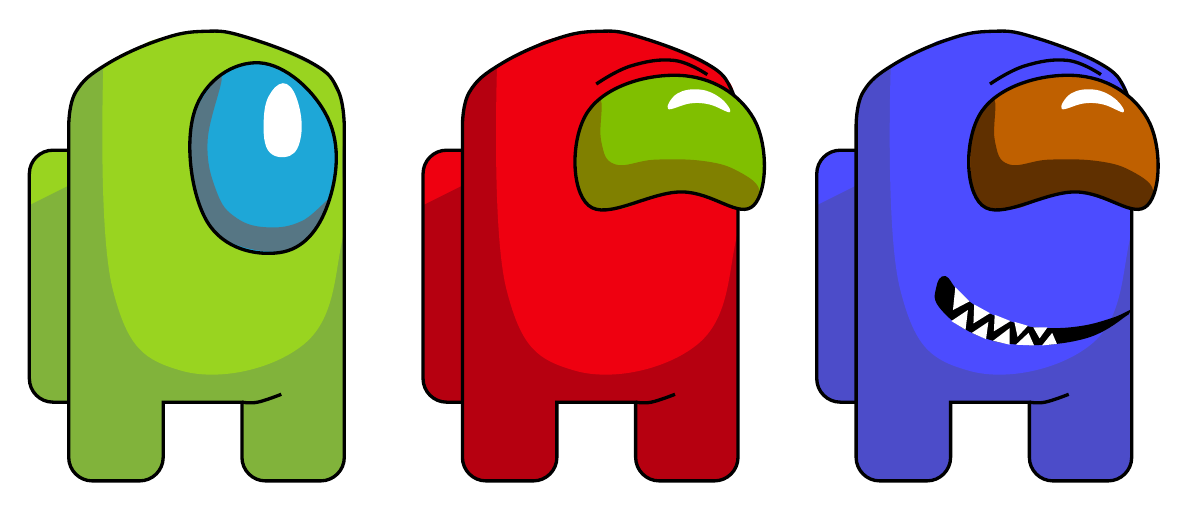
\begin{tikzpicture}[every path/.style={very thick}]
  \amongUsBackpackI{yellow!60!green}
  \amongUsBodyI{yellow!60!green}
  \amongUsEyesScaredI{cyan!90!red}

  \begin{scope}[shift={(5,0)}]
    \amongUsBackpackI{red!75!purple}
    \amongUsBodyI{red!75!purple}
    \amongUsEyesHappyI{green!50!orange}
  \end{scope}

  \begin{scope}[shift={(10,0)}]
    \amongUsBackpackI{blue!70!white}
    \amongUsBodyI{blue!70!white}
    \amongUsEyesHappyI{orange!75!black}
    \impostorSmile{black}
    \impostorTeeth{white}
  \end{scope}
\end{tikzpicture}
\end{FHZtcbAmongUs}

\subsection{That's a {\TikZ} impostor!}

Let's just create an example unifying impostor, hands and a crew member. The option \verb|xscale=-1| is used to create a mirror effect to draw the left hand from the original right hand design.\footnote{A future release might have starred options to directly insert left hands.}

\begin{FHZtcbAmongUs}[title=Watch out! That's a {\TikZ}-impostor!]
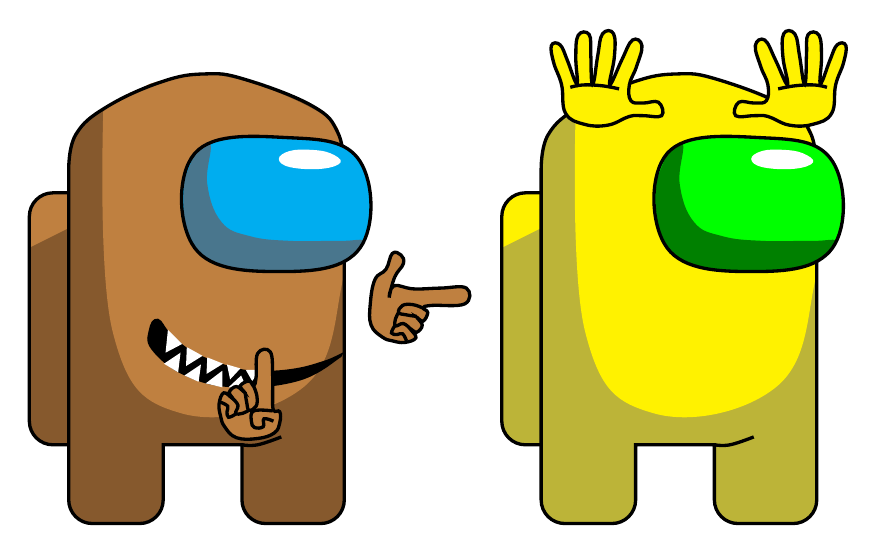
\begin{tikzpicture}[every path/.style={very thick}]
  \impostorI{brown}{cyan}{black}{white}
  \amongUsHandsF[shift={(3.75,-1)}, rotate around={270:(0.5,2.5)},
    xscale=-1]{brown}
  \amongUsHandsG[shift={(1.5,-1)}]{brown}
  \begin{scope}[shift={(6,0)}]
    \amongUsI{yellow}{green}
    \amongUsHandsB[shift={(0,3)}]{yellow}
    \amongUsHandsB[xscale=-1, shift={(-4,3)}]{yellow}
  \end{scope}
\end{tikzpicture}
\end{FHZtcbAmongUs}

\subsection{Oh no! Now you are a Ghost!}

The following commands draw the ectoplasmic body and the full ghost adding its eyes.
\begin{FHZtcbAmongUs}[listing only]
\amongUsGhostBodyI[<options>]{BodyColor}
\amongUsGhostI[<options>]{BodyColor}{EyeColor}
\end{FHZtcbAmongUs}
and also \texttt{Style II} versions.

After meeting the impostor at the last frame, you are now a ghost. And there are no excuses if you find a angry ghost floating around.
\begin{FHZtcbAmongUs}[title=Oh no! Now you are a Ghost!]

\begin{tikzpicture}[every path/.style={very thick}]
  \amongUsBackpackI{red!35!white}
  \amongUsGhostBodyI{red!35!white}
  \amongUsEyesAngryI{brown}

  \begin{scope}[shift={(5,0)}]
    \amongUsGhostI{purple}{orange!50!white}
    \amongUsHandsC[shift={(2,0)}]{purple}
    \amongUsHandsE[shift={(5,0)},xscale=-1]{purple}
  \end{scope}

  \begin{scope}[shift={(15,0)}, xscale=-1]
    \amongUsGhostI{green!50!blue}{yellow!50!black}
    \amongUsHandsA[shift={(1,0)}]{green!50!blue}
    \amongUsHandsB[shift={(5,0)},xscale=-1]{green!50!blue}
  \end{scope}
\end{tikzpicture}
\end{FHZtcbAmongUs}

\subsection{There is a Amoonguss among us}

The Pokémon named Amoonguss is a fungus whose name is very similar to the game, so that another artist create a fan art exploring this idea.
\begin{FHZtcbEnumerate}
  \item \href{https://www.reddit.com/r/AmongUs/comments/insse3/there_is_one_ditto_amoonguss/}{Reddit -- u/Sarasinapellido -- There is one ditto amoonguss}: Main discussion about the design.

  \begin{enumerate}
    \item \href{https://www.instagram.com/p/CEzs-cNKuQJ/}{Instagram -- leroleroart}: Original Amoonguss as among us design.
  \end{enumerate}
\end{FHZtcbEnumerate}

\begin{FHZtcbAmongUs}[title=There is one Ditto Amoonguss]
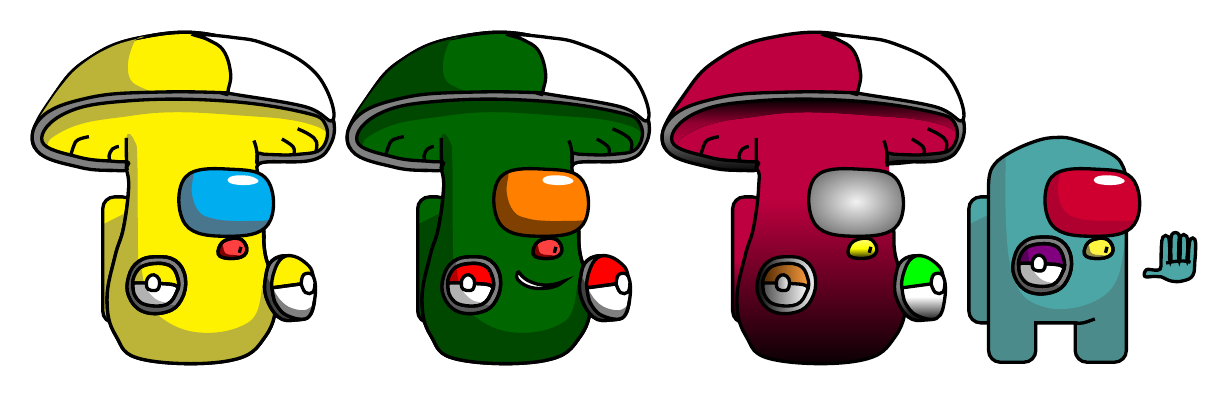
\begin{tikzpicture}[every path/.style={very thick}, scale=0.5]
  \amongUsBackpackI{yellow} 	 \amoongussBodyI{yellow}
  \amoongussNoseI{red} 				 \amoongussLeftHandI{yellow}
  \amoongussRightHandI{yellow} \amongUsEyesI{cyan}

  \amoongussI[shift={(8,0)}]{green!40!black}{orange}{red}{red}{red}
  \impostorSmile[shift={(9.5,1)}, scale=0.5]{white}

  \amoongussII[shift={(16,0)}]{purple}{gray}{green}{orange}{yellow}

  \begin{scope}[shift={(22,0)}]
    \amongUsI{teal!70}{red!25!purple}
    \amoongussNoseI{yellow}
    \amoongussRightHandI[shift={(0.5,0.5)}]{violet}
    \amongUsHandsA[shift={(5.5,0)},xscale=-1]{teal!70}
  \end{scope}
\end{tikzpicture}
\end{FHZtcbAmongUs}

\begin{FHZtcbAmongUs}[title=Wait! Is Amoonguss a ghost Pokémon?]
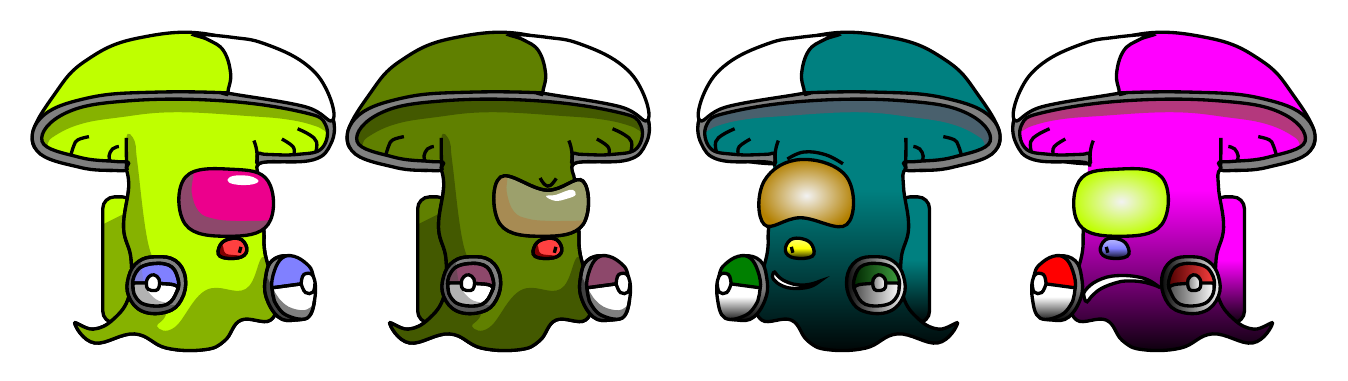
\begin{tikzpicture}[every path/.style={very thick}]
  \amoongussGhostI[scale=0.5]{lime}{magenta}
    {blue!50!white}{blue!50!white}{red}
  \begin{scope}[shift={(4,0)},scale=0.5]
    \amongUsBackpackI{lime!50!black}
    \amoongussGhostBodyI{lime!50!black}
    \amoongussNoseI{red}
    \amoongussLeftHandI{magenta!50!black}
    \amoongussRightHandI{magenta!50!black}
    \amongUsEyesAngryI{cyan!40!orange}
  \end{scope}
  \amoongussGhostII[shift={(14,0)},scale=0.5, xscale=-1]
  {magenta}{lime}{red}{red}{blue!50!white}
  \impostorSmile[shift={(11.8,1.8)}, scale=0.4, yscale=-1]{white}
  \begin{scope}[shift={(10,0)}, scale=0.5, xscale=-1]
    \amongUsBackpackII{cyan!50!black}
    \amoongussGhostBodyII{cyan!50!black}
    \amoongussNoseII{yellow}
    \amoongussLeftHandII{green!50!black}
    \amoongussRightHandII{green!50!black}
    \amongUsEyesHappyII{orange!40!olive}
    \impostorSmile[shift={(4,1)}, scale=0.5, xscale=-1]{white}
  \end{scope}
\end{tikzpicture}
\end{FHZtcbAmongUs}

\subsection{Don't forget Style II}

\texttt{Style II} should not be forget, and it also can be combined with ghost, hands and eyes emotions.
\begin{FHZtcbAmongUs}[title=Style II are looking back to you]

\begin{tikzpicture}[every path/.style={very thick}, scale=0.5, xscale=-1]
  \amongUsBackpackII{yellow} \amongUsBodyII{yellow}
  \amongUsEyesAngryII{cyan}  \impostorSmile{black}
  \impostorTeeth{white}
  \begin{scope}[shift={(6,0)}]
    \amongUsBackpackII{blue} \amongUsGhostBodyII{blue}
    \amongUsEyesHappyII{orange!75!black} \amongUsHandsE[shift={(2,0)}]{blue}
    \amongUsHandsG[shift={(3,1)}, xscale=-1, rotate around={90:(0,1)}]{blue}
  \end{scope}
  \begin{scope}[shift={(12,0)}]
    \amongUsBackpackII{red} \amongUsGhostBodyII{red}
    \amongUsEyesVeryangryII{violet}
    \impostorSmile{black} \impostorTeeth{white}
  \end{scope}
  \begin{scope}[shift={(17,0)}]
    \amongUsBackpackII{orange} \amongUsBodyII{orange}
    \amongUsEyesScaredII{blue}
    \amongUsHandsA{orange} \amongUsHandsD[shift={(4,0)}, xscale=-1]{orange}
  \end{scope}
  \amongUsGhostII[shift={(22,0)}]{lime}{red}
  \impostorII[shift={(27,0)}]{green!75!red}{gray}{black}{green}
\end{tikzpicture}
\end{FHZtcbAmongUs}

\subsection{Nice curves with Style III}

This style is based on the answer given by {\TeXStackExchange}'s User \textbf{hpekristiansen}. This style uses the command \textit{controls} instead of the smooth plot with given coordinates as Style I and II.

\begin{FHZtcbAmongUs}[title=Style III strikes amongUs]
  
\begin{tikzpicture}
    \amongUsIII{red}{blue}
    \amongUsIII[xscale=-1,shift={(-12,0)}]{yellow}{blue}
    \amongUsIII[shift={(12,0)},scale=0.5]{violet}{orange}
    \amongUsIII[scale=-0.5,shift={(-30,-16)}]{blue}{green}
  \end{tikzpicture}
\end{FHZtcbAmongUs}

\section{Using with own \texttt{.sty} file}

\subsection{Use as watermark}

The chosen package to add watermarks is
\begin{FHZtcbAmongUs}[listing only]
\usepackage{eso-pic}
\end{FHZtcbAmongUs}

A \texttt{.sty} file has been created to insert Among us characters from the package \texttt{tikz-among-us}, which syntax is
\begin{FHZtcbAmongUs}[listing only]
\usepackage[cor=<color>,<FG/BG>,type=<0/1>]{tikz-among-us-watermark-eso-pic}
\end{FHZtcbAmongUs}

The options are
\begin{FHZtcbEnumerate}
  \item cor=<color>
  \begin{itemize}
    \item default color is red
  \end{itemize}
  \item FG (default option) \textsl{OR} BG
  \begin{itemize}
    \item These options select between \texttt{{\textbackslash}AddToShipoutPictureFG} and \texttt{{\textbackslash}AddToShipoutPictureBG} from the package \texttt{eso-pic}.
  \end{itemize}
  \item type=<number>
  \begin{itemize}
    \item number can be either 0 (default if empty) for \texttt{Original Style} \textsf{OR} 1 for \texttt{Style I}. \texttt{Style II} has not been prepared, although any user can copy and edit the syntax at will.
  \end{itemize}
\end{FHZtcbEnumerate}

The package \texttt{kvoptions} have been used to provide flexible command with direct access to the options values in \texttt{cor} and \texttt{type}, and a simple true/false statement with \texttt{FG} and \texttt{BG}.
Any other kind or variation of watermark can be achieved by directing setting values to each \texttt{<parameter>} in:
\begin{FHZtcbAmongUs}[listing only]
\put(<X>,<Y>){\scalebox{<factor>}{\rotatebox{<degrees>}{\usebox\myboxAmongUs}}}
\end{FHZtcbAmongUs}
\noindent
where \texttt{{\textbackslash}myboxAmongUs} must be previously defined as
\begin{FHZtcbAmongUs}[listing only]
\myboxAmongUs\savebox\myboxAmongUs{%
  \tikz[color=<color>, opacity=<factor>]
    \node{\amongUsOriginal{<color>}{white}};
}
\end{FHZtcbAmongUs}

The following box presents some possible combinations of parameters which results are presented at \autoref{fig:fig_AmongUg}.
\begin{FHZtcbAmongUs}[listing only]
\usepackage{tikz-among-us-watermark-eso-pic}
\usepackage[FG]{tikz-among-us-watermark-eso-pic}
\usepackage[type=0]{tikz-among-us-watermark-eso-pic}

\usepackage[cor=blue]{tikz-among-us-watermark-eso-pic}
\usepackage[cor=green,FG]{tikz-among-us-watermark-eso-pic}

\usepackage[BG]{tikz-among-us-watermark-eso-pic}
\usepackage[cor=green!80!black,BG]{tikz-among-us-watermark-eso-pic}
\usepackage[cor=orange,type=0]{tikz-among-us-watermark-eso-pic}

\usepackage[cor=yellow!80!black,FG,type=0]{tikz-among-us-watermark-eso-pic}
\usepackage[cor=orange,BG,type=0]{tikz-among-us-watermark-eso-pic}
\usepackage[BG,type=1]{tikz-among-us-watermark-eso-pic}

\usepackage[cor=pink,type=1]{tikz-among-us-watermark-eso-pic}
\usepackage[cor=teal,FG,type=1]{tikz-among-us-watermark-eso-pic}
\usepackage[cor=brown,BG,type=1]{tikz-among-us-watermark-eso-pic}
\end{FHZtcbAmongUs}

\begin{figure}[htb] % [htpb]
  
\includegraphics[width = 0.20\linewidth]{Figuras/fig_AmongUs_01} \hfill
  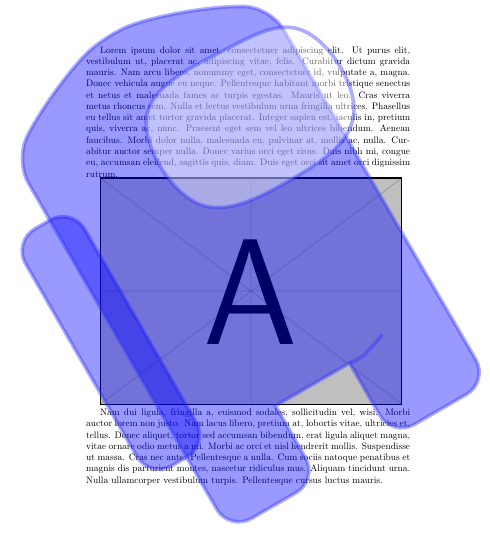
\includegraphics[width = 0.20\linewidth]{Figuras/fig_AmongUs_02} \hfill
  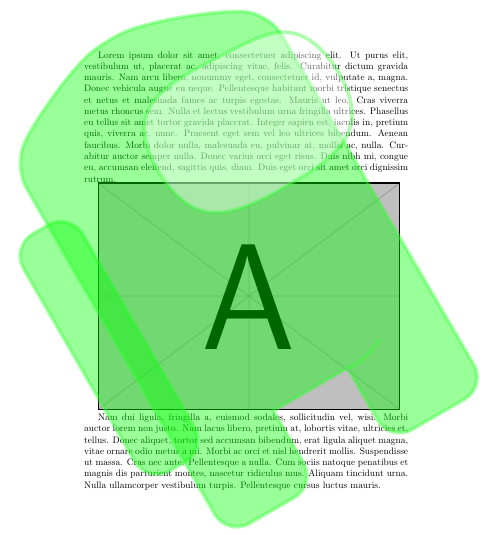
\includegraphics[width = 0.20\linewidth]{Figuras/fig_AmongUs_03} \hfill
  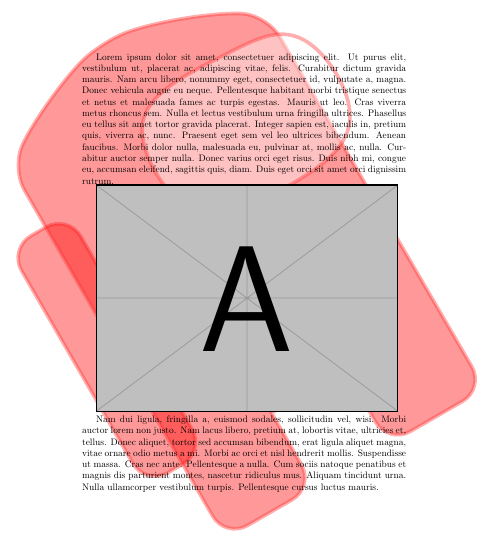
\includegraphics[width = 0.20\linewidth]{Figuras/fig_AmongUs_04} \\
  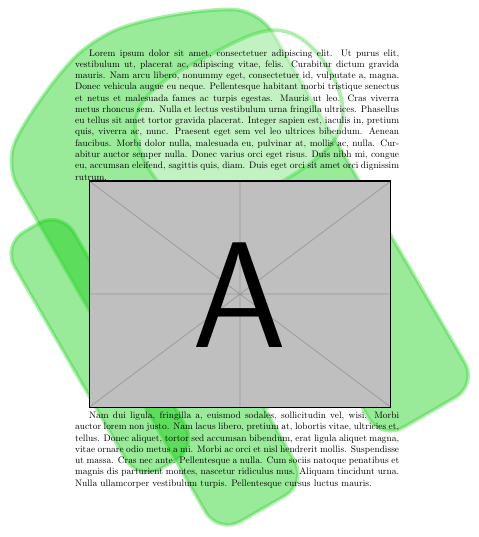
\includegraphics[width = 0.20\linewidth]{Figuras/fig_AmongUs_05} \hfill
  
\includegraphics[width = 0.20\linewidth]{Figuras/fig_AmongUs_06} \hfill
  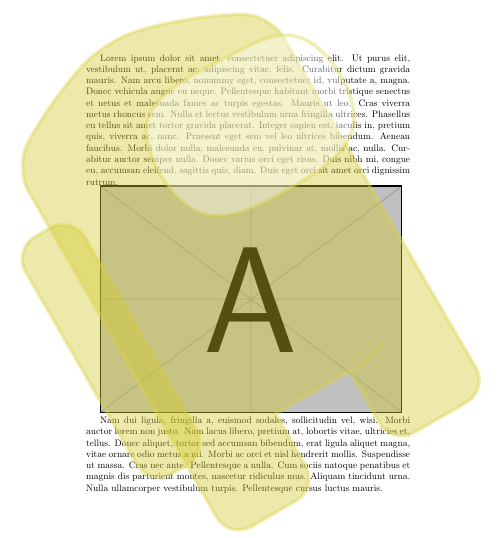
\includegraphics[width = 0.20\linewidth]{Figuras/fig_AmongUs_07} \hfill
  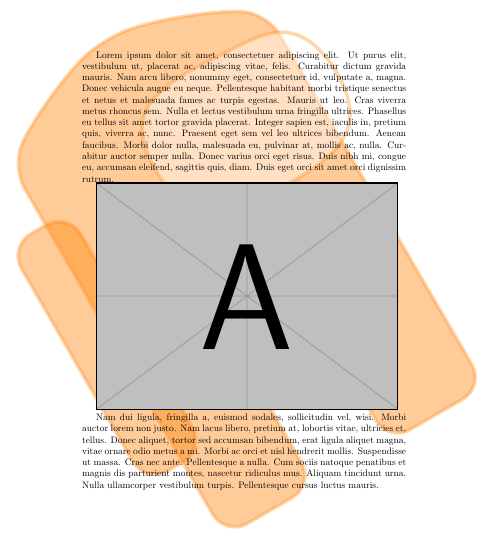
\includegraphics[width = 0.20\linewidth]{Figuras/fig_AmongUs_08} \\
% 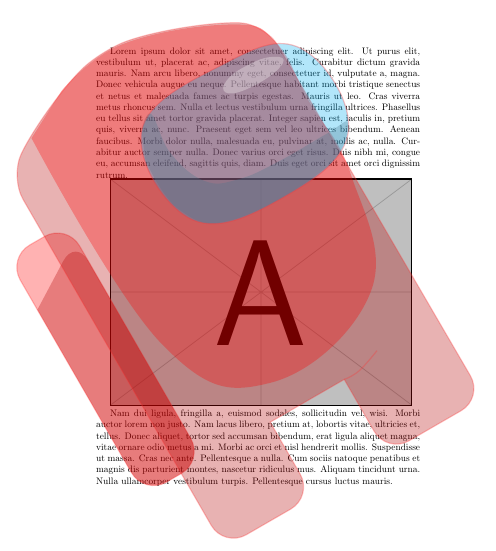
\includegraphics[width = 0.20\linewidth]{Figuras/fig_AmongUs_09} \\
  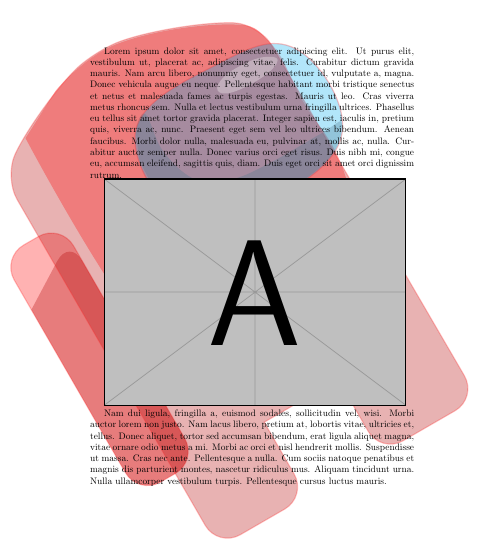
\includegraphics[width = 0.20\linewidth]{Figuras/fig_AmongUs_10} \hfill
  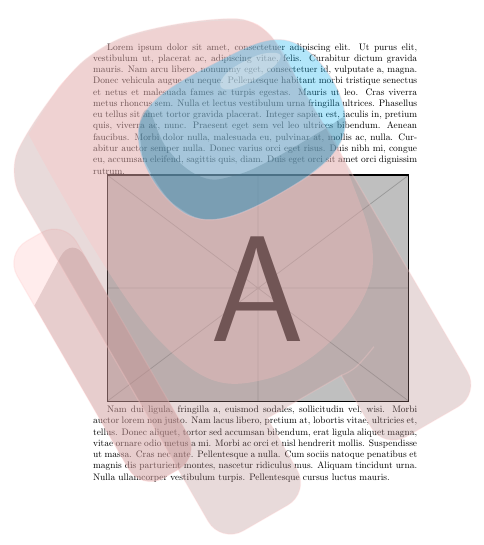
\includegraphics[width = 0.20\linewidth]{Figuras/fig_AmongUs_11} \hfill
  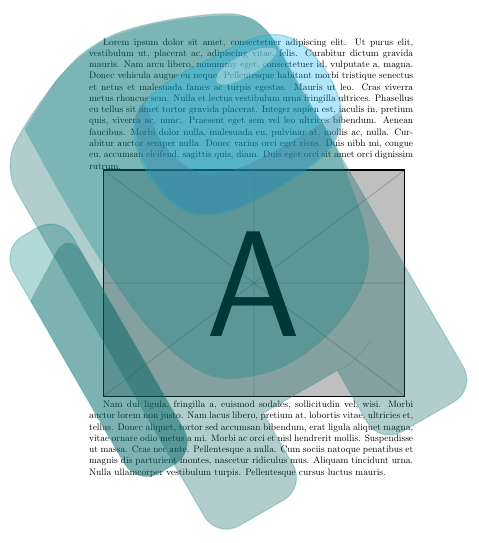
\includegraphics[width = 0.20\linewidth]{Figuras/fig_AmongUs_12} \hfill
  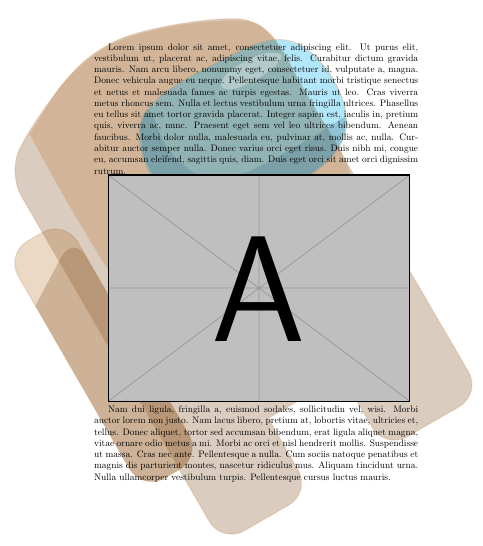
\includegraphics[width = 0.20\linewidth]{Figuras/fig_AmongUs_13}
  \caption{Example of each presented combination of watermark}
  \label{fig:fig_AmongUg}
\end{figure}

The selected combination used in this documentation is
\begin{FHZtcbAmongUs}[listing only]
\usepackage[cor=violet!70!white,BG,type=1]{tikz-among-us-watermark-eso-pic}
\end{FHZtcbAmongUs}

\subsection{Use as page number}

The required packages are:
\begin{FHZtcbAmongUs}[listing only]
\usepackage{fancyhdr}
\end{FHZtcbAmongUs}
The package \texttt{fancyhdr} enables the user to edit headers and footers. I present a simple possibility to use the Among us characters in the footer of each page, such as the ones in this documentation.

The central core of the idea is to shift the position of the \verb|\amongUsI|, scale it to match its center around the displacement of the command \verb|\thepage| -- that inserts the page's number -- and \texttt{rotate around} using some math to rotate to body around its center.
In the example below, it turns 45 degrees each new page, creating the idea of a body floating around.

The following command just changes the footer. To apply other options check the package \texttt{fancyhdr}.
\begin{FHZtcbAmongUs}[listing only]
\fancyfoot[RO,LE]{%
  
\begin{tikzpicture}
    \amongUsI[rotate around={45*(\thepage-1):(1.75,2.3)},
      scale=0.25, shift={(5,7)}]{yellow}{cyan}
    \node at (1.75,2.3) {\thepage};
  \end{tikzpicture}
}
\end{FHZtcbAmongUs}

\section{Using inside other packages}

\subsection{Use as watermark in tcolorbox}

The package \texttt{tcolorbox} is one of the most versatile packages of all {\LaTeX}. One of its feature is the possibility to create boxes with many styles, including boxes with watermarks as presented in page 174 of the \texttt{tcolorbox} manual (\texttt{/tcb/watermark tikz)}.
\begin{FHZtcbAmongUs}[listing only]
\usepackage{tcolorbox}
\end{FHZtcbAmongUs}

The very implementation used in this report to create enumerated list with some Among us floating around is:
\begin{FHZtcbAmongUs}[listing only]
\newtcolorbox{FHZboxEnumerateStyle}{
  enhanced,
  colback=orange!15!white,
  colframe=orange!50!black,
  watermark tikz={\tikz
    \node[opacity=0.4, rotate around={-45:(1.75,2.3)}]
      {\amongUsOriginal{blue}{white}};
    \node[opacity=0.4, rotate around={45:(1.75,2.3)}] at (5,0)
      {\amongUsOriginal{pink}{white}};
    \node[opacity=0.4, rotate around={-135:(1.75,2.3)}] at (10,0)
      {\amongUsOriginal{green}{white}};
    \node[opacity=0.4, rotate around={135:(1.75,2.3)}] at (15,0)
      {\amongUsOriginal{olive}{white}{black}{white}};
  }
}
\newenvironment{FHZtcbEnumerate}{%
  \begin{FHZboxEnumerateStyle}\begin{enumerate}}
    {\end{enumerate}\end{FHZboxEnumerateStyle}
}
\end{FHZtcbAmongUs}

\begin{FHZtcbEnumerate}
  \item This is an example of a \texttt{enumerate} list inside a \texttt{tcolorbox} with \texttt{tikz-among-us} as watermark.
\end{FHZtcbEnumerate}


\subsection{Use as animation}

This example uses the following package
\begin{FHZtcbAmongUs}[listing only]
\usepackage{animate}
\end{FHZtcbAmongUs}

This example creates a variable from 0 to 360 to represent each degree of a full rotation.\footnote{Animation requires some PDF visualization software to properly work. Internet browsers are not normally suitable for this task.} Four Among us characters are placed around the screen by using the option \texttt{shift={(x0,y0)}} and then rotating them around each respective center of mass. In order to achieve this effect, the most left command must be \texttt{shift} and then \texttt{rotate around}, the opposite order will rotate around the given point by will shift the object relative center of rotation. To make a body rotate in the opposite direction it is just necessary to add a minus sign in front of the angle variable. Animation is present in \autoref{fig:anim_floating_around}.
\begin{FHZtcbAmongUs}[listing only]
\begin{animateinline}[controls,loop]{30}
  \multiframe{180}{rt=0+1}{%
    \begin{tikzpicture}
      \draw (-2,-10) rectangle (15,7);
      \useasboundingbox (-2,-10) rectangle (15,7);
      \amoongussI[shift={(\rt/9-2.5,-3)}, scale=0.3]
        {purple!40!black}{yellow}{green}{green}{red}
      \amongUsI[rotate around={2*\rt:(2,3)}]
        {orange}{blue}
      \amongUsGhostI[shift={(8,0)}, rotate around={-2*\rt:(2,3)}]
        {cyan}{orange}
      \amongUsII[shift={(0,-8)}, rotate around={2*\rt:(2,3)}]
        {red}{gray}
      \impostorI[shift={(8,-8)}, rotate around={-2*\rt:(2,3)}]
        {green!50!black}{cyan}{black}{white}
    \end{tikzpicture}
  }
\end{animateinline}
\end{FHZtcbAmongUs}


\begin{figure}[ht!]
  \begin{animateinline}[controls,loop]{30}
    \multiframe{180}{rt=0+1}{%
      \begin{tikzpicture}
        \draw (-2,-10) rectangle (15,7);
        \useasboundingbox (-2,-10) rectangle (15,7);
        \amoongussI[shift={(\rt/9-2.5,-3)}, scale=0.3]
          {purple!40!black}{yellow}{green}{green}{red}
        \amongUsI[rotate around={2*\rt:(2,3)}]
          {orange}{blue}
        \amongUsGhostI[shift={(8,0)}, rotate around={-2*\rt:(2,3)}]
          {cyan}{orange}
        \amongUsII[shift={(0,-8)}, rotate around={2*\rt:(2,3)}]
          {red}{gray}
        \impostorI[shift={(8,-8)}, rotate around={-2*\rt:(2,3)}]
          {green!50!black}{cyan}{black}{white}
      \end{tikzpicture}
    }
  \end{animateinline}
  \caption{Example of a floating around animation}
  \label{fig:anim_floating_around}
\end{figure}

\section{Future features and ideas}

\begin{FHZtcbEnumerate}
  \item Add options for hands $\checkmark$
  \item Add options to different emotions through the eyes in styles I $\checkmark$ and II $\checkmark$
  \item Improve scale method $\checkmark$
  \item Draw a impostor design $\checkmark$
  \item Draw maps
  \item Create left and right hand options
  \begin{enumerate}
    \item Create a starred version of right hands as left hands
  \end{enumerate}
  \item Add other emotions than ``angry'' ones
  \begin{enumerate}
    \item Happy $\checkmark$
    \item Scared $\checkmark$
  \end{enumerate}
  \item Create ghost design $\checkmark$
  \item Create Pokémon Amoonguss design $\checkmark$
\end{FHZtcbEnumerate}

\section{Historic and version}

\begin{FHZtcbEnumerate}[leftmargin=3.5cm]
  \item[1.0.0 (2020-10-20):] Publication of the style with the original design and Styles I and II of shadows.
  \item[1.0.1 (2020-10-23):] Minor typos have been corrected.
  \item[1.1.0 (2020-10-31):] Added new features (both \texttt{Styles})
    \begin{itemize}[leftmargin=-2cm]
      \item Hands;
      \item Eyes with emotions (Angry, Very angry, Happy, Scared);
      \item Impostor parts and full body;
      \item Ghost body;
      \item Pokémon Amoonguss parts and full body;
      \item \texttt{rounded corners} removed to improve \texttt{scale};
      \item Ghost Amoonguss body.
    \end{itemize}

  \item[1.2.0 (2021-10-27):] Added Style III.
\end{FHZtcbEnumerate}

\section{Implementation}

\subsection{tikz-among-us.sty}

\autoref{alg:tikz-among-us} shows the implementation of the package \texttt{tikz-among-us.sty}.

% -----------------------------
%, lastline = 10, firstnumber = 1, nolol, style = estiloExemAzul/Verm/Verd
\lstinputlisting[firstline = 5,  firstnumber = 1, label = {alg:tikz-among-us}, caption = {Package implementation}, style = estiloExemVerd]
{C:/Users/FHZ/Dropbox/LaTeX_pacotes/tex/latex/tikz-among-us/tikz-among-us.sty}
% -----------------------------

\subsection{tikz-among-us-fancyhdr.sty}

\autoref{alg:tikz-among-us-fancyhdr} shows the implementation of the package \texttt{tikz-among-us-fancyhdr.sty}.

% -----------------------------
% firstline = 1, lastline = 10, firstnumber = 1, nolol, style = estiloExemAzul/Verm/Verd
\lstinputlisting[firstline = 5,  firstnumber = 1, label = {alg:tikz-among-us-fancyhdr}, caption = {Package implementation}, style = estiloExemVerd]
{C:/Users/FHZ/Dropbox/LaTeX_pacotes/tex/latex/tikz-among-us/tikz-among-us-fancyhdr.sty}
% -----------------------------

\subsection{tikz-among-us-watermark-eso-pic.sty}

\autoref{alg:tikz-among-us-watermark-eso-pic} shows the implementation of the package \texttt{tikz-among-us-watermark-eso-pic.sty}.

% -----------------------------
% firstline = 1, lastline = 10, firstnumber = 1, nolol, style = estiloExemAzul/Verm/Verd
\lstinputlisting[firstline = 5,  firstnumber = 1, label = {alg:tikz-among-us-watermark-eso-pic}, caption = {Package implementation}, style = estiloExemVerd]
{C:/Users/FHZ/Dropbox/LaTeX_pacotes/tex/latex/tikz-among-us/tikz-among-us-watermark-eso-pic.sty}
% -----------------------------

\end{document}